
% \begin{table}[t!]
\footnotesize
\centering
\caption{Case report identification performance per diagnosis and aggregated across all diagnoses.}
\label{tab:case_report_identification}
% \begin{adjustbox}{max width=0.95\textwidth}
\begin{tabular}{llcccc}
\toprule
Subset & Diagnosis & Precision & Recall & Accuracy & F1 Score \\
\midrule
\multirow{6}{*}{PubMed metadata} 
    & Atrial Fibrillation & 0.84 & 0.94 & 0.80 & 0.89 \\
    & COVID-19            & 0.94 & 0.89 & 0.85 & 0.92 \\
    & Diabetes            & 0.85 & 1.00 & 0.85 & 0.92 \\
    & Hypertension        & 1.00 & 1.00 & 1.00 & 1.00 \\
    & Sepsis              & 0.95 & 0.95 & 0.90 & 0.95 \\
\cmidrule(lr){2-6}
    & \textbf{All Diagnoses} & \text{0.92} & \textbf{0.96} & \text{0.88} & \text{0.94} \\
\midrule
\multirow{6}{*}{LLM-Pipeline}
    & Atrial Fibrillation & 1.00 & 1.00 & 1.00 & 1.00 \\
    & COVID-19            & 1.00 & 0.89 & 0.90 & 0.94 \\
    & Diabetes            & 1.00 & 0.94 & 0.95 & 0.97 \\
    & Hypertension        & 1.00 & 0.95 & 0.95 & 0.97 \\
    & Sepsis              & 1.00 & 1.00 & 1.00 & 1.00 \\
\cmidrule(lr){2-6}
    & \textbf{All Diagnoses} & \textbf{1.00} & \textbf{0.96} & \textbf{0.96} & \textbf{0.98} \\
\bottomrule
\end{tabular}
% \end{adjustbox}
\vspace{-5mm}
\end{table}



% \begin{table}[!ht]
%     \footnotesize
%     \centering
%     \caption{Case report identification performance per diagnosis}
%     \label{tab:diagnosis_results}
%     \begin{tabular}{l l c c c c c}
%         \hline
%         Subset & Diagnosis & Sensitivity & Specificity & Accuracy & Precision & F1 Score \\
%         \hline
%         PubMed MetaData  & Atrial Fibrillation & 0.94 & 0.00 & 0.80 & 0.84 & 0.89 \\
%         LLM-Pipeline     & Atrial Fibrillation & 1.00 & 1.00 & 1.00 & 1.00 & 1.00 \\
%         \hline
%         PubMed MetaData  & COVID-19           & 0.89 & 0.00 & 0.85 & 0.94 & 0.92 \\
%         LLM-Pipeline     & COVID-19           & 0.89 & 1.00 & 0.90 & 1.00 & 0.94 \\
%         \hline
%         PubMed MetaData  & Diabetes           & 1.00 & 0.00 & 0.85 & 0.85 & 0.92 \\
%         LLM-Pipeline     & Diabetes           & 0.94 & 1.00 & 0.95 & 1.00 & 0.97 \\
%         \hline
%         PubMed MetaData  & Hypertension       & 1.00 & 0.00 & 1.00 & 1.00 & 1.00 \\
%         LLM-Pipeline     & Hypertension       & 0.95 & 0.00 & 0.95 & 1.00 & 0.97 \\
%         \hline
%         PubMed MetaData  & Sepsis             & 0.95 & 0.00 & 0.90 & 0.95 & 0.95 \\
%         LLM-Pipeline     & Sepsis             & 1.00 & 1.00 & 1.00 & 1.00 & 1.00 \\
%         \hline
%     \end{tabular}
% \end{table}

% \begin{table}[!ht]
%     \footnotesize
%     \centering
%     \caption{Aggregated case report identification performance across all diagnoses}
%     \label{tab:aggregated_results}
%     \begin{tabular}{l c c c c c}
%         \hline
%         Subset & Sensitivity & Specificity & Accuracy & Precision & F1 Score \\
%         \hline
%         PubMed MetaData  & \textbf{0.96} & 0.00 & 0.88 & 0.92 & 0.94 \\
%         LLM-Pipeline     & \textbf{0.96} & \textbf{1.00} & \textbf{0.96} & \textbf{1.00} & \textbf{0.98} \\
%         \hline
%     \end{tabular}
% \end{table}
\vspace{-2mm}
\subsection{Demographic Characterization of PMOA-TTS}
\label{sec:demographics}
\vspace{-2mm}

% For diagnosis extraction, the LLM was prompted to act as an expert physician and return a list of patient-specific diagnoses from the report, clearly distinguishing true diagnoses (e.g., “acne,” “DRESS syndrome”) from general clinical findings (e.g., “rash,” “leukocytosis”). The prompt directed the model to list the primary diagnosis first, include one diagnosis per line, and omit any explanatory text (full prompt in Appendix \ref{apd:diagnosis_prompt}).

For demographic extraction, we used an LLM-based query to retrieve age, sex, and ethnicity to characterize the demographic composition of the corpus. The prompt specified that age be reported in years, sex as Male, Female, a custom string, or Not Specified, and ethnicity according to U.S. Census categories or as Not Specified (see Appendix \ref{apd:demographics_prompt}).

Our analysis shows a median age of 47 years, with age distribution peaks at 5-year intervals, indicating rounding in clinical reporting (Figure \ref{fig:flowchart}). The gender distribution is balanced (52\% male, 47\% female, and 1\% with unspecified gender.) Most case reports (89\%) do not specify the patient's ethnicity. When ethnicity is specified, White/Caucasian (5\%) and Asian (3\%) are the most common, followed by African (1\%) and Other (2\%). Compared to U.S. population demographics, Asian patients are overrepresented, likely due to the international scope of PubMed publications.

% DEMOGRAPHICS
% # In 10.000 sample,
% # 52 % male, 47 % female, 1% not specified
% # US Census ethnicity
% #   89 % Not Specified
% #    5 % White/Caucasian
% #    3 % Asian
% #    1 % African
% #    2 % Other

%%%%%%%%%%%%%%%%%%%%%%%%%%%%%%%%%%%%%%%%%%%%
% \noindent
% \begin{minipage}[t]{\textwidth}
%     \begin{minipage}[t]{0.48\columnwidth}
%         \centering
%         % \begin{figure}[htb]
%         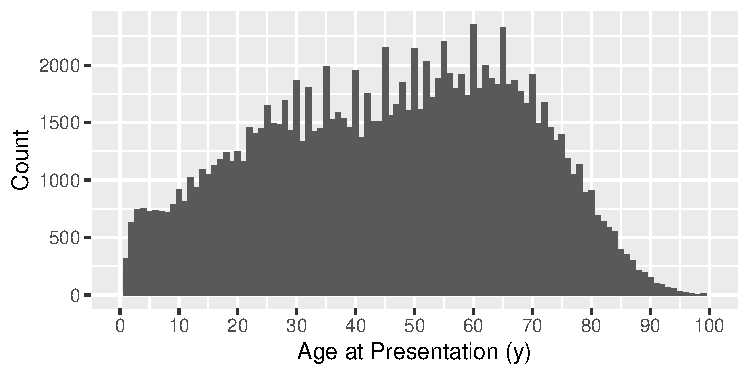
\includegraphics[width=\columnwidth]{Plots_tables/125k_age.pdf}
%         % \captionof{figure}{Histogram of Age (years) in the PMOA 20\% sample.}
%         % \label{fig:age}
%         % \end{figure}
%     \end{minipage}
%     \hfill
%     \begin{minipage}[t]{0.48\columnwidth}
%         \vspace*{-18em}
%         \centering
%         % \begin{table}[h]
% \caption{Demographic characteristics of the PMOA 10,000 sample}
% \captionof{table}{Demographic characteristics of the PMOA 10,000 sample}
% \label{tab:demographics}
\vspace{0.5em}
\centering
\begin{tabular}{l r}
\toprule
\textbf{Characteristic} & \textbf{Percent (\%)} \\
\midrule
\multicolumn{2}{l}{\textbf{Sex}} \\
\quad Male & 52 \\
\quad Female & 47 \\
\quad Not Specified & 1 \\
\midrule
\multicolumn{2}{l}{\textbf{Ethnicity}} \\
\quad White/Caucasian & 5 \\
\quad Asian & 3 \\
\quad African & 1 \\
\quad Other & 2 \\
\quad Not Specified & 89 \\
\bottomrule
\end{tabular}
% \end{table}
%     \end{minipage}
%     \captionof{figure}{Age, sex, and ethnicity of the PMOA TTS corpus.}
%     \label{fig:demographics}
% \end{minipage}
%%%%%%%%%%%%%%%%%%%%%%%%%%%%%%%%%%%%%%%%%%%%

\vspace{-1.5mm}
\subsection{Case Report Identification Performance}
\label{sec:results_case_identification}

% \begin{table}[t!]
\footnotesize
\centering
\caption{Case report identification performance per diagnosis and aggregated across all diagnoses.}
\label{tab:case_report_identification}
% \begin{adjustbox}{max width=0.95\textwidth}
\begin{tabular}{llcccc}
\toprule
Subset & Diagnosis & Precision & Recall & Accuracy & F1 Score \\
\midrule
\multirow{6}{*}{PubMed metadata} 
    & Atrial Fibrillation & 0.84 & 0.94 & 0.80 & 0.89 \\
    & COVID-19            & 0.94 & 0.89 & 0.85 & 0.92 \\
    & Diabetes            & 0.85 & 1.00 & 0.85 & 0.92 \\
    & Hypertension        & 1.00 & 1.00 & 1.00 & 1.00 \\
    & Sepsis              & 0.95 & 0.95 & 0.90 & 0.95 \\
\cmidrule(lr){2-6}
    & \textbf{All Diagnoses} & \text{0.92} & \textbf{0.96} & \text{0.88} & \text{0.94} \\
\midrule
\multirow{6}{*}{LLM-Pipeline}
    & Atrial Fibrillation & 1.00 & 1.00 & 1.00 & 1.00 \\
    & COVID-19            & 1.00 & 0.89 & 0.90 & 0.94 \\
    & Diabetes            & 1.00 & 0.94 & 0.95 & 0.97 \\
    & Hypertension        & 1.00 & 0.95 & 0.95 & 0.97 \\
    & Sepsis              & 1.00 & 1.00 & 1.00 & 1.00 \\
\cmidrule(lr){2-6}
    & \textbf{All Diagnoses} & \textbf{1.00} & \textbf{0.96} & \textbf{0.96} & \textbf{0.98} \\
\bottomrule
\end{tabular}
% \end{adjustbox}
\vspace{-5mm}
\end{table}



% \begin{table}[!ht]
%     \footnotesize
%     \centering
%     \caption{Case report identification performance per diagnosis}
%     \label{tab:diagnosis_results}
%     \begin{tabular}{l l c c c c c}
%         \hline
%         Subset & Diagnosis & Sensitivity & Specificity & Accuracy & Precision & F1 Score \\
%         \hline
%         PubMed MetaData  & Atrial Fibrillation & 0.94 & 0.00 & 0.80 & 0.84 & 0.89 \\
%         LLM-Pipeline     & Atrial Fibrillation & 1.00 & 1.00 & 1.00 & 1.00 & 1.00 \\
%         \hline
%         PubMed MetaData  & COVID-19           & 0.89 & 0.00 & 0.85 & 0.94 & 0.92 \\
%         LLM-Pipeline     & COVID-19           & 0.89 & 1.00 & 0.90 & 1.00 & 0.94 \\
%         \hline
%         PubMed MetaData  & Diabetes           & 1.00 & 0.00 & 0.85 & 0.85 & 0.92 \\
%         LLM-Pipeline     & Diabetes           & 0.94 & 1.00 & 0.95 & 1.00 & 0.97 \\
%         \hline
%         PubMed MetaData  & Hypertension       & 1.00 & 0.00 & 1.00 & 1.00 & 1.00 \\
%         LLM-Pipeline     & Hypertension       & 0.95 & 0.00 & 0.95 & 1.00 & 0.97 \\
%         \hline
%         PubMed MetaData  & Sepsis             & 0.95 & 0.00 & 0.90 & 0.95 & 0.95 \\
%         LLM-Pipeline     & Sepsis             & 1.00 & 1.00 & 1.00 & 1.00 & 1.00 \\
%         \hline
%     \end{tabular}
% \end{table}

% \begin{table}[!ht]
%     \footnotesize
%     \centering
%     \caption{Aggregated case report identification performance across all diagnoses}
%     \label{tab:aggregated_results}
%     \begin{tabular}{l c c c c c}
%         \hline
%         Subset & Sensitivity & Specificity & Accuracy & Precision & F1 Score \\
%         \hline
%         PubMed MetaData  & \textbf{0.96} & 0.00 & 0.88 & 0.92 & 0.94 \\
%         LLM-Pipeline     & \textbf{0.96} & \textbf{1.00} & \textbf{0.96} & \textbf{1.00} & \textbf{0.98} \\
%         \hline
%     \end{tabular}
% \end{table}

\begin{table}[t!]
    \footnotesize
    \centering
    \caption{Case report identification performance per diagnosis and aggregated across all diagnoses.}
    \label{tab:combined_diagnosis_results}
    \begin{adjustbox}{max width=0.74\textwidth}
    \begin{tabular}{llcccc}
        \toprule
        Subset & Diagnosis & Precision & Recall & Accuracy & F1 Score \\
        \midrule
        \multirow{6}{*}{PubMed MetaData} 
            & Atrial Fibrillation & 0.84 & 0.94 & 0.80 & 0.89 \\
            & COVID-19            & 0.94 & 0.89 & 0.85 & 0.92 \\
            & Diabetes            & 0.85 & 1.00 & 0.85 & 0.92 \\
            & Hypertension        & 1.00 & 1.00 & 1.00 & 1.00 \\
            & Sepsis              & 0.95 & 0.95 & 0.90 & 0.95 \\
        \cmidrule(lr){2-6}
            & \textbf{All Diagnoses} & \text{0.92} & \textbf{0.96} & \text{0.88} & \text{0.94} \\
        \midrule
        \multirow{6}{*}{LLM-Pipeline}
            & Atrial Fibrillation & 1.00 & 1.00 & 1.00 & 1.00 \\
            & COVID-19            & 1.00 & 0.89 & 0.90 & 0.94 \\
            & Diabetes            & 1.00 & 0.94 & 0.95 & 0.97 \\
            & Hypertension        & 1.00 & 0.95 & 0.95 & 0.97 \\
            & Sepsis              & 1.00 & 1.00 & 1.00 & 1.00 \\
        \cmidrule(lr){2-6}
            & \textbf{All Diagnoses} & \textbf{1.00} & \textbf{0.96} & \textbf{0.96} & \textbf{0.98} \\
        \bottomrule
    \end{tabular}
    \end{adjustbox}
    \vspace{-5pt}
\end{table}

Our evaluation of case report identification methods compared our LLM-Pipeline approach against PubMed's metadata-based filtering across five different diagnoses: Diabetes, Sepsis, Hypertension, COVID-19, and Atrial Fibrillation. 
Using clinician-assigned labels as ground truth, we computed precision, recall, accuracy, and F1 score for each approach.

The LLM-Pipeline approach demonstrates superior performance with perfect precision (1.00) across all diagnostic categories and also aggregated across all diagnoses (Table~\ref{tab:combined_diagnosis_results}), indicating that when our pipeline identifies a document as a single-patient case report, it is always correct. In contrast, the PubMed MetaData approach shows more variable precision, ranging from 0.84 for Atrial Fibrillation to 1.00 for Hypertension, with an overall precision of 0.92.

Both methods achieve similar recall (0.96), indicating comparable success in identifying true case reports.
However, the LLM-Pipeline attains higher overall accuracy (0.96 vs. 0.88), reflecting its superior ability to distinguish both true positives and true negatives. This accuracy gain is largely due to the LLM-Pipeline’s effectiveness in excluding non-single-patient reports, which the PubMed MetaData approach often misclassifies.

Examining performance by diagnostic category reveals that both approaches perform best on Sepsis and Hypertension cases, while showing more variability with Atrial Fibrillation, COVID-19, and Diabetes reports. The LLM-Pipeline maintains consistently high performance across all categories, with F1 scores ranging from 0.94 to 1.00. These findings highlight the significant improvements in precision and overall classification quality offered by our LLM-Pipeline approach for case report identification, ensuring that the PMOA-TTS corpus contains high-quality, single-patient case reports with minimal contamination from multi-patient or non-case report documents.


%%%%%%%%%%%%%%%%%%%%%%%%%%%%%%%%%%%%%%%%%%%%%%%
%%%%%%%%%%%%%%%%%%%%%%%%%%%%%%%%%%%%%%%%%%%%%%
% \subsection{Comparing LLM annotated TTS with PMOA metadata}

% To evaluate the performance of our case report identification approach, we compare our LLM-Pipeline to PubMed MetaData, where we curated a dataset of 100 reports across 5 different diagnoses: Diabetes, Sepsis, Hypertension, COVID-19, and Atrial Fibrillation.

% The selection process was as follows:
% \begin{itemize}
%     \item We used LLaMA to generate a diagnosis for each report identified by the LLM-Pipeline approach. Among the top 10 most frequently occurring diagnoses, we selected five and randomly picked 10 reports for each diagnosis.
%     \item For PubMed MetaData, we used the case report filter on PubMed and ensured that the selected reports were present in the December 17, 2024, PubMed Open Access subset. Similarly, we selected 10 reports per diagnosis.
%     \item The reports from the two approaches were ensured to be unique, resulting in a total of 100 reports (20 for each diagnosis, with 10 from LLM-Pipeline and 10 from PubMed MetaData).
%     \item A clinician manually reviewed each report and labeled the number of case reports present. A report was labeled as 1 if it contained exactly one case report and 0 if it contained none or more than one.
% \end{itemize}

% In evaluating the performance of the LLM-pipeline approach, we used clinician-assigned labels as the ground truth and computed several classification metrics. Sensitivity was calculated as the proportion of correctly identified case reports, while specificity represented the proportion of correctly identified non-case reports. Accuracy was defined as the overall proportion of correct classifications. Precision was determined as the proportion of predicted case reports that were correct. Finally, the F1 score, which is the harmonic mean of precision and sensitivity, was also computed to provide a balanced measure of the model's performance.

% Table~\ref{tab:diagnosis_results} presents the classification performance for each diagnosis. The LLM-Pipeline approach achieves perfect or near-perfect performance across all diagnoses, with sensitivity and specificity values of 1.00 in multiple cases. In contrast, the PubMed MetaData approach demonstrates high sensitivity but lacks specificity, frequently misclassifying non-case reports as case reports.

% Table~\ref{tab:aggregated_results} aggregates results across all diagnoses. The LLM-Pipeline approach achieves an overall accuracy of 0.96, compared to 0.88 for the PubMed MetaData approach. Notably, LLM-Pipeline achieves a specificity of 1.00, correctly rejecting all non-case reports, while PubMed MetaData has a specificity of 0.00, indicating it misclassified all non-case reports as positive. The precision of LLM-Pipeline is 1.00, ensuring that all detected case reports are true positives, whereas PubMed MetaData achieves a precision of 0.92.

% These findings highlight the improved precision and specificity of our LLM-Pipeline approach for case report identification.
% \begin{table}[t!]
\footnotesize
\centering
\caption{Case report identification performance per diagnosis and aggregated across all diagnoses.}
\label{tab:case_report_identification}
% \begin{adjustbox}{max width=0.95\textwidth}
\begin{tabular}{llcccc}
\toprule
Subset & Diagnosis & Precision & Recall & Accuracy & F1 Score \\
\midrule
\multirow{6}{*}{PubMed metadata} 
    & Atrial Fibrillation & 0.84 & 0.94 & 0.80 & 0.89 \\
    & COVID-19            & 0.94 & 0.89 & 0.85 & 0.92 \\
    & Diabetes            & 0.85 & 1.00 & 0.85 & 0.92 \\
    & Hypertension        & 1.00 & 1.00 & 1.00 & 1.00 \\
    & Sepsis              & 0.95 & 0.95 & 0.90 & 0.95 \\
\cmidrule(lr){2-6}
    & \textbf{All Diagnoses} & \text{0.92} & \textbf{0.96} & \text{0.88} & \text{0.94} \\
\midrule
\multirow{6}{*}{LLM-Pipeline}
    & Atrial Fibrillation & 1.00 & 1.00 & 1.00 & 1.00 \\
    & COVID-19            & 1.00 & 0.89 & 0.90 & 0.94 \\
    & Diabetes            & 1.00 & 0.94 & 0.95 & 0.97 \\
    & Hypertension        & 1.00 & 0.95 & 0.95 & 0.97 \\
    & Sepsis              & 1.00 & 1.00 & 1.00 & 1.00 \\
\cmidrule(lr){2-6}
    & \textbf{All Diagnoses} & \textbf{1.00} & \textbf{0.96} & \textbf{0.96} & \textbf{0.98} \\
\bottomrule
\end{tabular}
% \end{adjustbox}
\vspace{-5mm}
\end{table}



% \begin{table}[!ht]
%     \footnotesize
%     \centering
%     \caption{Case report identification performance per diagnosis}
%     \label{tab:diagnosis_results}
%     \begin{tabular}{l l c c c c c}
%         \hline
%         Subset & Diagnosis & Sensitivity & Specificity & Accuracy & Precision & F1 Score \\
%         \hline
%         PubMed MetaData  & Atrial Fibrillation & 0.94 & 0.00 & 0.80 & 0.84 & 0.89 \\
%         LLM-Pipeline     & Atrial Fibrillation & 1.00 & 1.00 & 1.00 & 1.00 & 1.00 \\
%         \hline
%         PubMed MetaData  & COVID-19           & 0.89 & 0.00 & 0.85 & 0.94 & 0.92 \\
%         LLM-Pipeline     & COVID-19           & 0.89 & 1.00 & 0.90 & 1.00 & 0.94 \\
%         \hline
%         PubMed MetaData  & Diabetes           & 1.00 & 0.00 & 0.85 & 0.85 & 0.92 \\
%         LLM-Pipeline     & Diabetes           & 0.94 & 1.00 & 0.95 & 1.00 & 0.97 \\
%         \hline
%         PubMed MetaData  & Hypertension       & 1.00 & 0.00 & 1.00 & 1.00 & 1.00 \\
%         LLM-Pipeline     & Hypertension       & 0.95 & 0.00 & 0.95 & 1.00 & 0.97 \\
%         \hline
%         PubMed MetaData  & Sepsis             & 0.95 & 0.00 & 0.90 & 0.95 & 0.95 \\
%         LLM-Pipeline     & Sepsis             & 1.00 & 1.00 & 1.00 & 1.00 & 1.00 \\
%         \hline
%     \end{tabular}
% \end{table}

% \begin{table}[!ht]
%     \footnotesize
%     \centering
%     \caption{Aggregated case report identification performance across all diagnoses}
%     \label{tab:aggregated_results}
%     \begin{tabular}{l c c c c c}
%         \hline
%         Subset & Sensitivity & Specificity & Accuracy & Precision & F1 Score \\
%         \hline
%         PubMed MetaData  & \textbf{0.96} & 0.00 & 0.88 & 0.92 & 0.94 \\
%         LLM-Pipeline     & \textbf{0.96} & \textbf{1.00} & \textbf{0.96} & \textbf{1.00} & \textbf{0.98} \\
%         \hline
%     \end{tabular}
% \end{table}

%%%%%%%%%%%%%%%%%%%%%%%%%%%%%%%%%%%%%%%%%%%%%%%%%%%%%%
%%%%%%%%%%%%%%%%%%%%%%%%%%%%%%%%%%%%%%%%%%%%%%%%%%%%%

\subsection{Evaluation of Clinical Textual Time Series Quality}

We evaluated the quality of extracted textual time series using the manually annotated subset as ground truth, comparing seven LLM variants: DeepSeek-R1, DeepSeek-R1-UD-IQ1, DeepSeek-V3-0324, LLaMA 3.3 70B, OpenAI O1, OpenAI O3, and OpenAI O4-mini. A comparison of different LLM annotations and sensitivity to different prompt strategies can be found in Appendices \ref{apd:example_annotations} and \ref{apd:prompt_ablation} respectively.

%\subsubsection{Text Event Match Performance}

\textbf{Text Event Match Performance.} Figure~\ref{fig:tts_evaluation} (left) shows the cumulative density of cosine distances between model-generated and reference event descriptions. A threshold of 0.1 (vertical line) defines a successful match. DeepSeek-R1 (black) and its quantized variant DeepSeek-R1-UD-IQ1 (orange) outperform other models, with ~80\% of aligned events falling below the threshold. DeepSeek-V3-0324 (light blue) and O4-mini (red) form a second tier, while LLaMA 3.3 70B (green), O1 (light yellow), and O3 (blue) show more dispersed distributions, with only 70\% of events below the threshold. These analyses highlights clear differences in how well models generate event descriptions that align semantically with expert annotations. The strong performance of DeepSeek-R1 and its quantized variant indicates their enhanced ability to model clinical language patterns found in case reports.

%\subsubsection{Temporal Ordering Performance}

\textbf{Temporal Ordering Performance.} Using the cosine distance threshold to identify matched events, we assessed temporal ordering accuracy via the concordance index (c-index).
As shown in Figure~\ref{fig:tts_evaluation} (right), LLaMA 3.3 70B achieves the highest median c-index (0.96), with DeepSeek-V3-0324 and DeepSeek-R1 following closely.

The relationship between event matching and concordance evaluation is important to consider. Models applying stricter matching thresholds may appear to perform better on concordance by evaluating only the most confidently matched events. In contrast, models matching a broader set of events—including more ambiguous cases—encounter a more difficult ordering task. LLaMA 3.3 70B’s strong performance in temporal ordering is notable given its lower match rate, suggesting it effectively captures relative timing even when its textual matches are less precise.
Appendix \ref{apd:choosing_match_threshold} discusses how adjusting the event match threshold allows tuning the balance between match coverage and ordering accuracy.

%\subsubsection{Time Discrepancy Analysis}

\textbf{Time Discrepancy Analysis.} Figure~\ref{fig:tts_evaluation} (left) displays the cumulative probability distribution of time differences (log-scaled) between predicted and reference timestamps, illustrating each model’s timestamping accuracy.
DeepSeek-R1 (black line) shows the steepest curve, indicating that a higher proportion of its predictions are temporally close to the reference points. In contrast, LLaMA 3.3 70B (green line) produces a flatter curve, reflecting greater variation and lower precision in absolute time prediction. The right panel in Figure \ref{fig:tts_evaluation} breaks down performance across time intervals—presentation, 1 hour, 1 day, 1 week, 1 year, and beyond. All models perform well for events near the presentation time, but their accuracy declines as the temporal distance increases. DeepSeek models consistently show stronger performance across intervals, whereas LLaMA 3.3 70B exhibits more noticeable degradation for distant events.

Taken together, this analysis highlights a key distinction: while LLaMA 3.3 70B is more effective at predicting relative event order (concordance), DeepSeek models—particularly DeepSeek-R1—are better at assigning precise timestamps, even for events far from the reference point.


% \subsection{Evaluation of clinical textual time-series}

% We assessed the textual time-series extracted from PMOA case reports with 3 metrics: event match rate, concordance (c-index) and log-time discrepancy.  The physician annotations of the twenty cases from \cite{frattallone2024using,wang2025large} were used as ground truth.

% \subsubsection{Text event match}

% A recursive best-match procedure has been previously employed to align predicted and reference clinical findings \cite{wang2025large}. In this approach, event matches are determined based on string similarity to minimize many-to-one (surjective) mappings. For each reference event, the predicted event with the lowest distance is selected, with event order used to resolve ties. Once a match is established, both the reference and predicted events are removed, and the procedure is repeated recursively on the remaining items. Several distance metrics were evaluated, including Levenshtein distance, cosine distance between BERT (bert-base-uncased) embeddings, and cosine distance between sentence embeddings from PubMedBERT (S-PubMedBert-MS-MARCO). Based on prior manual evaluation, the PubMedBERT-based distance with a cosine similarity threshold of 0.1 was found to yield the most reliable matches and was adopted for this work.

% The textual alignment of predicted clinical findings were evaluated with respect to manual annotations by a clinical expert across five LLM variants (Figure \ref{fig:cosine_distance_density} left). The cumulative density of cosine distances indicates that DeepSeek-R1 and DeepSeek-R1-UD-IQ1 yield the highest proportion of low-distance matches, with over 80\% of aligned events falling below the 0.1 threshold (Figure \ref{fig:cosine_distance_density}, left), suggesting strong semantic similarity to the reference annotations. In comparison, models like LLaMA3-70B and O1 produce more dispersed distributions, indicating less accurate matching. 

% \subsubsection{Temporal ordering}

% Among the matched events, we then analyzed their temporal ordering and discrepancies between labeled and predicted timestamps. To quantify this, we used the concordance index (c-index), which measures the probability that a randomly selected pair of predicted findings is correctly ordered in time. Higher c-index values indicate better alignment with the reference timeline. The results (Figure \ref{fig:cosine_distance_density}, right) show that the DeepSeek variants consistently achieve the highest temporal coherence, with median c-index values above 0.95. This indicates strong agreement with the reference event sequences and reinforces the models’ ability to capture both the textual content and temporal structure of clinical findings.

% Further, we evaluated the accuracy of temporal ordering by analyzing the discrepancies between labeled and predicted timestamps. The log-time discrepancy was computed as $log(1 + \Delta t)$, where $\Delta t$  represents the absolute time difference (in hours) between predicted and reference timestamps. Cumulative time discrepancy plots were generated to illustrate the proportion of cases falling below specific thresholds.

% To assess timestamp accuracy, cumulative distributions of log-scaled time differences between predicted and reference event times were analyzed. DeepSeek variants, particularly DeepSeek-R1, achieve steeper cumulative curves, indicating that a larger proportion of events are predicted with minimal temporal error across scales ranging from hour to year (Figure \ref{fig:time_difference}, left). In contrast, L3.3 70B and DeepSeek-R1-UD-IQ1 show flatter curves, reflecting greater variability in timestamp predictions. When stratified by reference time intervals, the DeepSeek models consistently maintain tighter alignment across all bins, while performance for L3.3 and O1 deteriorates more noticeably as the distance from the reference point increases (Figure \ref{fig:time_difference}, right). These findings highlight the ability of DeepSeek models to reconstruct clinical timelines with both fine-grained and long-range temporal precision.


% \begin{figure}[!htbp]
%   \centering
%   % Scale the entire 2x2 block (caption stays normal size)
%   \resizebox{0.6\linewidth}{!}{%
%     \begin{minipage}{\linewidth}
%       % ---------- Row 1 ----------
%       \begin{minipage}[t]{.48\linewidth}\vspace{0pt}\centering
%         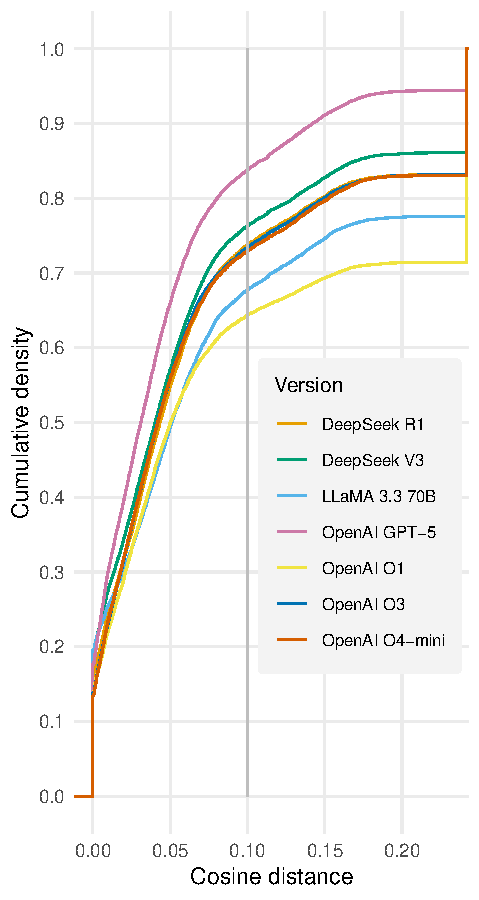
\includegraphics[page=1, width=\linewidth]{Plots_tables/pmoa_updated_man_figs.pdf}
%       \end{minipage}\hfill
%       \begin{minipage}[t]{.48\linewidth}\vspace{0pt}\centering
%         \includegraphics[page=2, width=\linewidth]{Plots_tables/pmoa_updated_man_figs.pdf}
%       \end{minipage}

%       \vspace{4pt} % space between rows (adjust as needed)

%       % ---------- Row 2 ----------
%       \begin{minipage}[t]{.48\linewidth}\vspace{0pt}\centering
%         \includegraphics[page=3, width=\linewidth]{Plots_tables/pmoa_updated_man_figs.pdf}
%       \end{minipage}\hfill
%       \begin{minipage}[t]{.48\linewidth}\vspace{0pt}\centering
%         \includegraphics[page=4, width=\linewidth]{Plots_tables/pmoa_updated_man_figs.pdf}
%       \end{minipage}
%     \end{minipage}%
%   }
%   \caption{Event match cumulative distribution (top left), concordance box plots (top right), log-time discrepancy overall (bottom left), and log-time discrepancy stratified by annotator timestamp (bottom right).}
%   \label{fig:tts_evaluation}
%   \vspace{-5mm}
% \end{figure}



\begin{figure}[!tbp]
\centering
    \begin{minipage}[t]{0.242\textwidth}
    \centering
    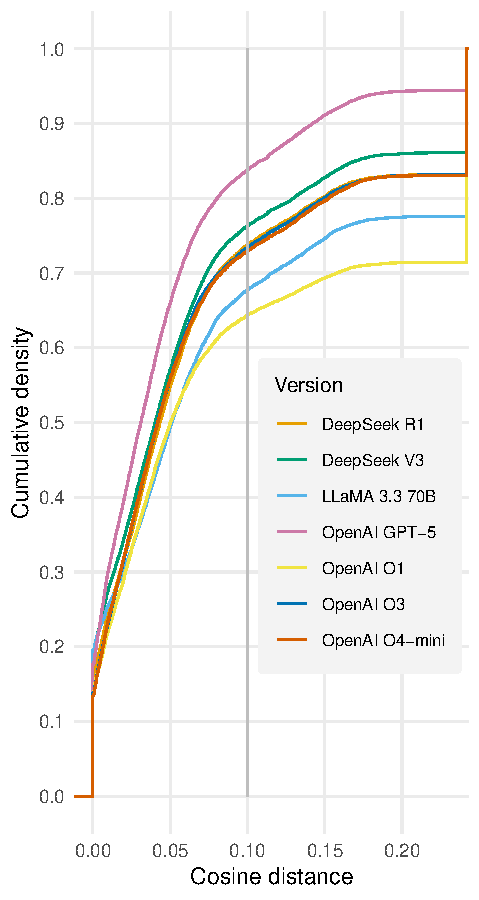
\includegraphics[page=1, width=\linewidth]{Plots_tables/pmoa_updated_man_figs.pdf}
    \end{minipage}
    \hfill
    \begin{minipage}[t]{0.242\textwidth}
    \centering
    \includegraphics[page=2, width=\linewidth]{Plots_tables/pmoa_updated_man_figs.pdf}
    \end{minipage}
    \hfill
    \begin{minipage}[t]{0.242\textwidth}
    \centering
    \includegraphics[page=3, width=\linewidth]{Plots_tables/pmoa_updated_man_figs.pdf}
    \end{minipage}
    \hfill
    \begin{minipage}[t]{0.242\textwidth}
    \centering
    \includegraphics[page=4, width=\linewidth]{Plots_tables/pmoa_updated_man_figs.pdf}
    \end{minipage}
    \caption{Comparison of different LLM for extracting temporal clinical events from case reports. From left to right: (\textbf{A}) event match cumulative distribution function, (\textbf{B}) concordance box plots, (\textbf{C}) time discrepancy from manual annotation timestamps among matched events (overall), and (\textbf{D}) time discrepancy disaggregated by clinician annotator timestamp (time from presentation). 
    %\textcolor{red}{Have same figure for LAPJV?}
    }
    \label{fig:tts_evaluation}
    \vspace{-10pt}
\end{figure}

% \begin{figure}
%     \centering
%     \begin{minipage}{0.4\textwidth}
%         \centering
%         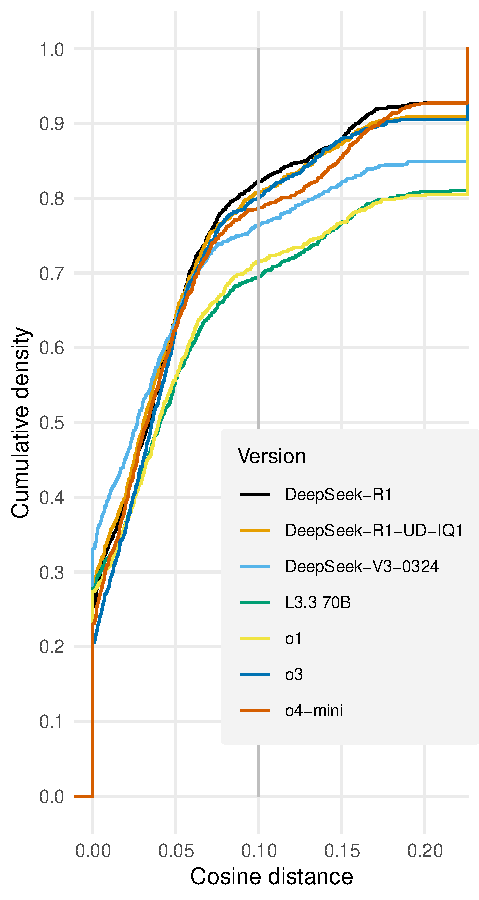
\includegraphics[width=\linewidth]{Plots_tables/pmoa241217_man_o34_figs_Part1.pdf} 
%         % \caption{}
%     \end{minipage}
%     \begin{minipage}{0.4\textwidth}
%         \centering
%         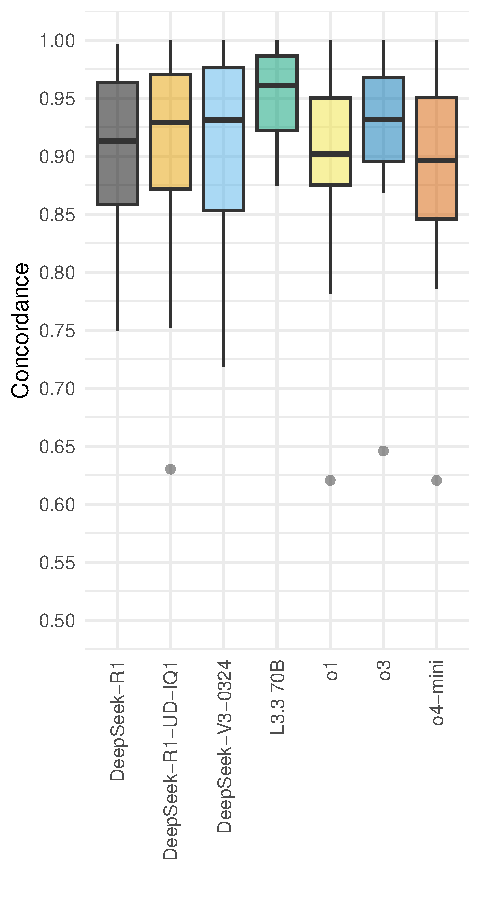
\includegraphics[width=\linewidth]{Plots_tables/pmoa241217_man_o34_figs_Part2.pdf} 
%         % \caption{}
%     \end{minipage}
%     \caption{Cumulative density plot of cosine distance, illustrating textual similarity between model outputs and reference annotations across three model versions. A steeper curve at lower distances indicates better event matching (left). Concordance index (c-index) boxplot comparing the temporal ordering accuracy of event predictions among DeepSeek-R1, DeepSeek-R1-UD-IQ1, DeepSeek-V3-0324-UD-IQ1, L3.3 70B-Instruct, and O1. Higher values reflect better alignment with reference event sequences (right).}
%     \label{fig:cosine_distance_density}
% \end{figure}

% %Plots_tables/pmoa241217_man_o34_figs_Part3.pdf

% \begin{figure}
%     \centering
%     \begin{minipage}{0.4\textwidth}
%         \centering
%         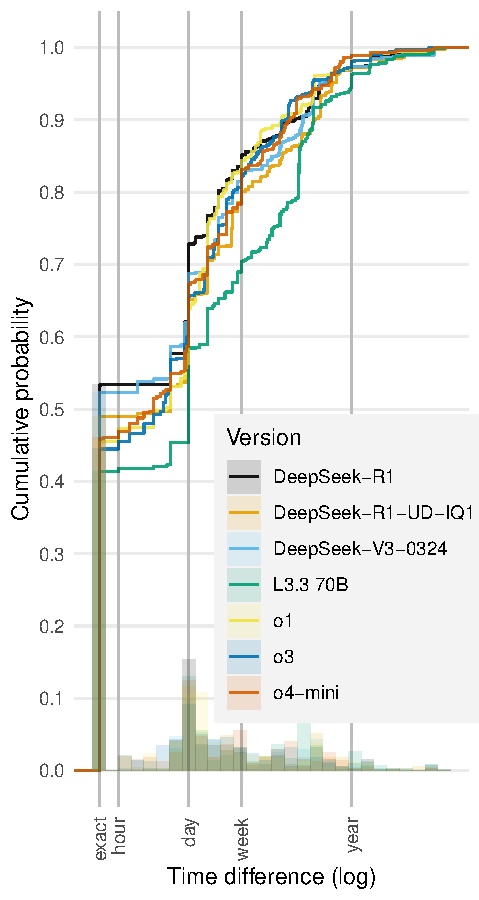
\includegraphics[width=\linewidth]{Plots_tables/pmoa241217_man_o34_figs_Part3.pdf}
%         % \caption{}
%     \end{minipage}
%     % \hfill
%     \begin{minipage}{0.4\textwidth}
%         \centering
%         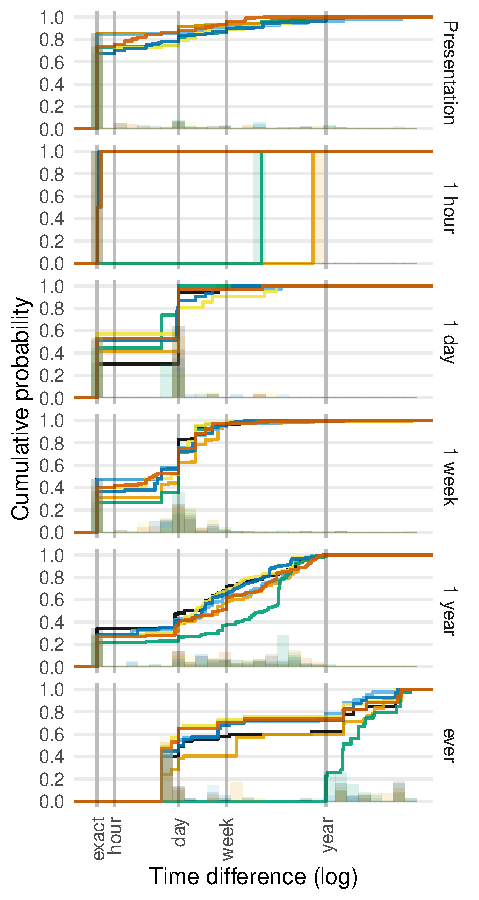
\includegraphics[width=\linewidth]{Plots_tables/pmoa241217_man_o34_figs_Part4.pdf}
%         % \caption{}
%     \end{minipage}
%     \caption{Cumulative probability plot of time differences (log-scaled), showing the proportion of events captured within various time thresholds. Steeper curves at shorter time discrepancies indicate higher precision in temporal alignment (left). Stratified time discrepancy analysis across different time intervals (hour, day, week, year). The distribution highlights increasing errors for events further removed from the reference timestamp (right).}
%     \label{fig:time_difference}
% \end{figure}


\subsection{Diagnosis Distribution Analysis}

Additionally, we prompted the LLM to act as an expert physician and list patient-specific diagnoses from the report, distinguishing true diagnoses (e.g., “acne,” “DRESS syndrome”) from general clinical findings (e.g., “rash,” “leukocytosis”). The prompt instructed the model to list the primary diagnosis first, include one diagnosis per line, and omit explanatory text (full prompt in Appendix \ref{apd:diagnosis_prompt}).

To assess the medical coverage of our corpus, we analyzed the diagnoses extracted through this LLM-based method, as detailed in Appendix~\ref{apd:umls_mapping}. Figure~\ref{fig:top_diagnoses} shows the 20 most frequent diagnoses, demonstrating the broad clinical scope of the dataset. Hypertensive disorders, including hypertensive disease, diastolic and systolic hypertension, prehypertension, and renal hypertension, are the most common, followed by diabetes mellitus and its subtypes.

This distribution aligns with the prevalence of chronic conditions typically seen in clinical practice, particularly cardiovascular, metabolic, and renal disorders, and matches the corpus’s demographic profile, with a median patient age of 45 years—an age group commonly affected by these conditions.

We also examined diagnosis co-occurrence patterns using a clustered heatmap (Figure~\ref{fig:diagnosis_cooccurrence}), revealing strong groupings of related conditions. Notably, hypertensive spectrum disorders and diabetes variants cluster together, reflecting well-established clinical links, such as those between diabetes and chronic kidney disease, or atrial fibrillation and hypertension.

This analysis highlights the diverse range of medical conditions in the PMOA-TTS corpus and demonstrates its suitability for clinical prediction tasks across multiple disease domains.



\begin{figure}[!tb]
    % \vspace{-5pt}
    \centering
    \quad
    \begin{subfigure}[t]{0.44\textwidth}
        \centering
        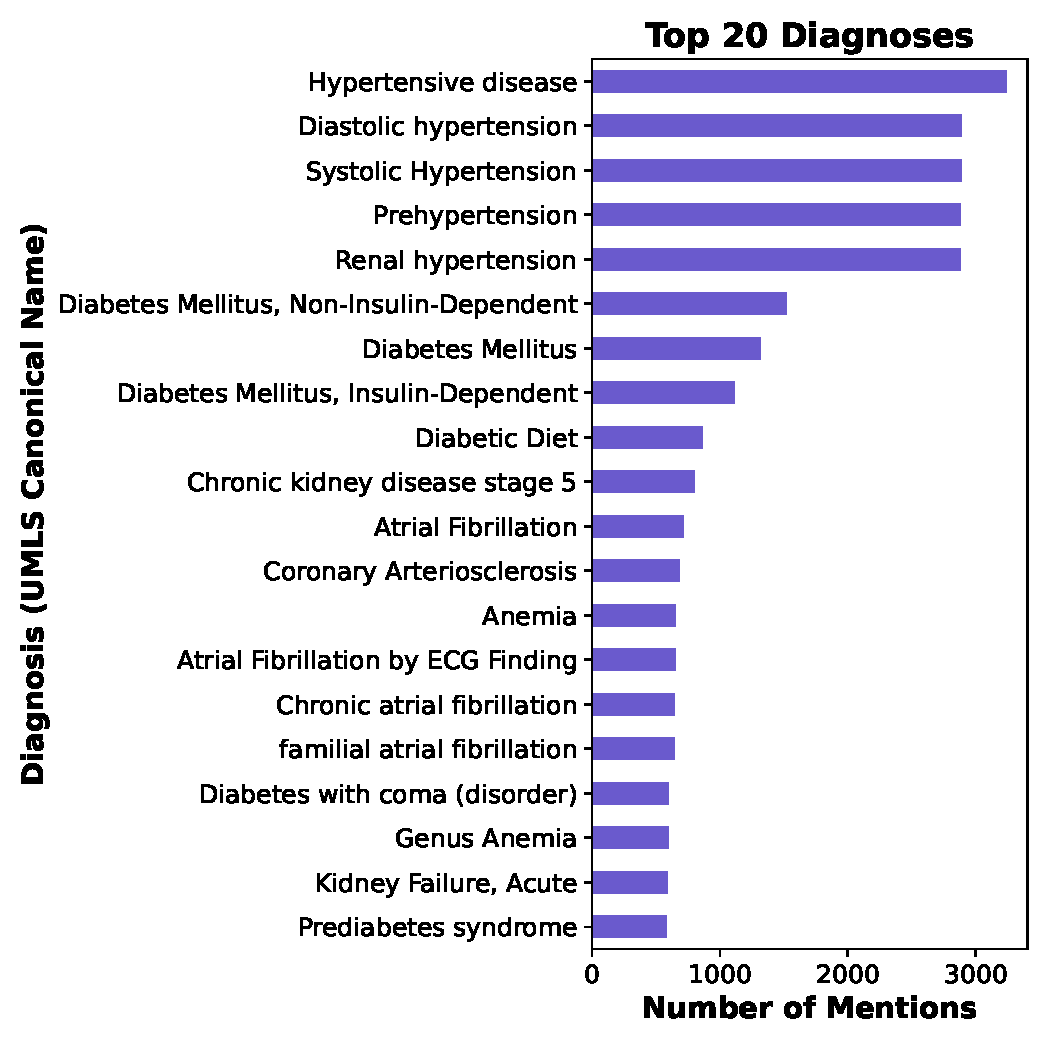
\includegraphics[width=0.99\linewidth]{Plots_tables/top_diagnoses_umls.pdf}
        \caption{Most Frequent Diagnoses in PMOA-TTS}
        \label{fig:top_diagnoses}
    \end{subfigure}
    \hfill
    \begin{subfigure}[t]{0.49\textwidth}
        \centering
        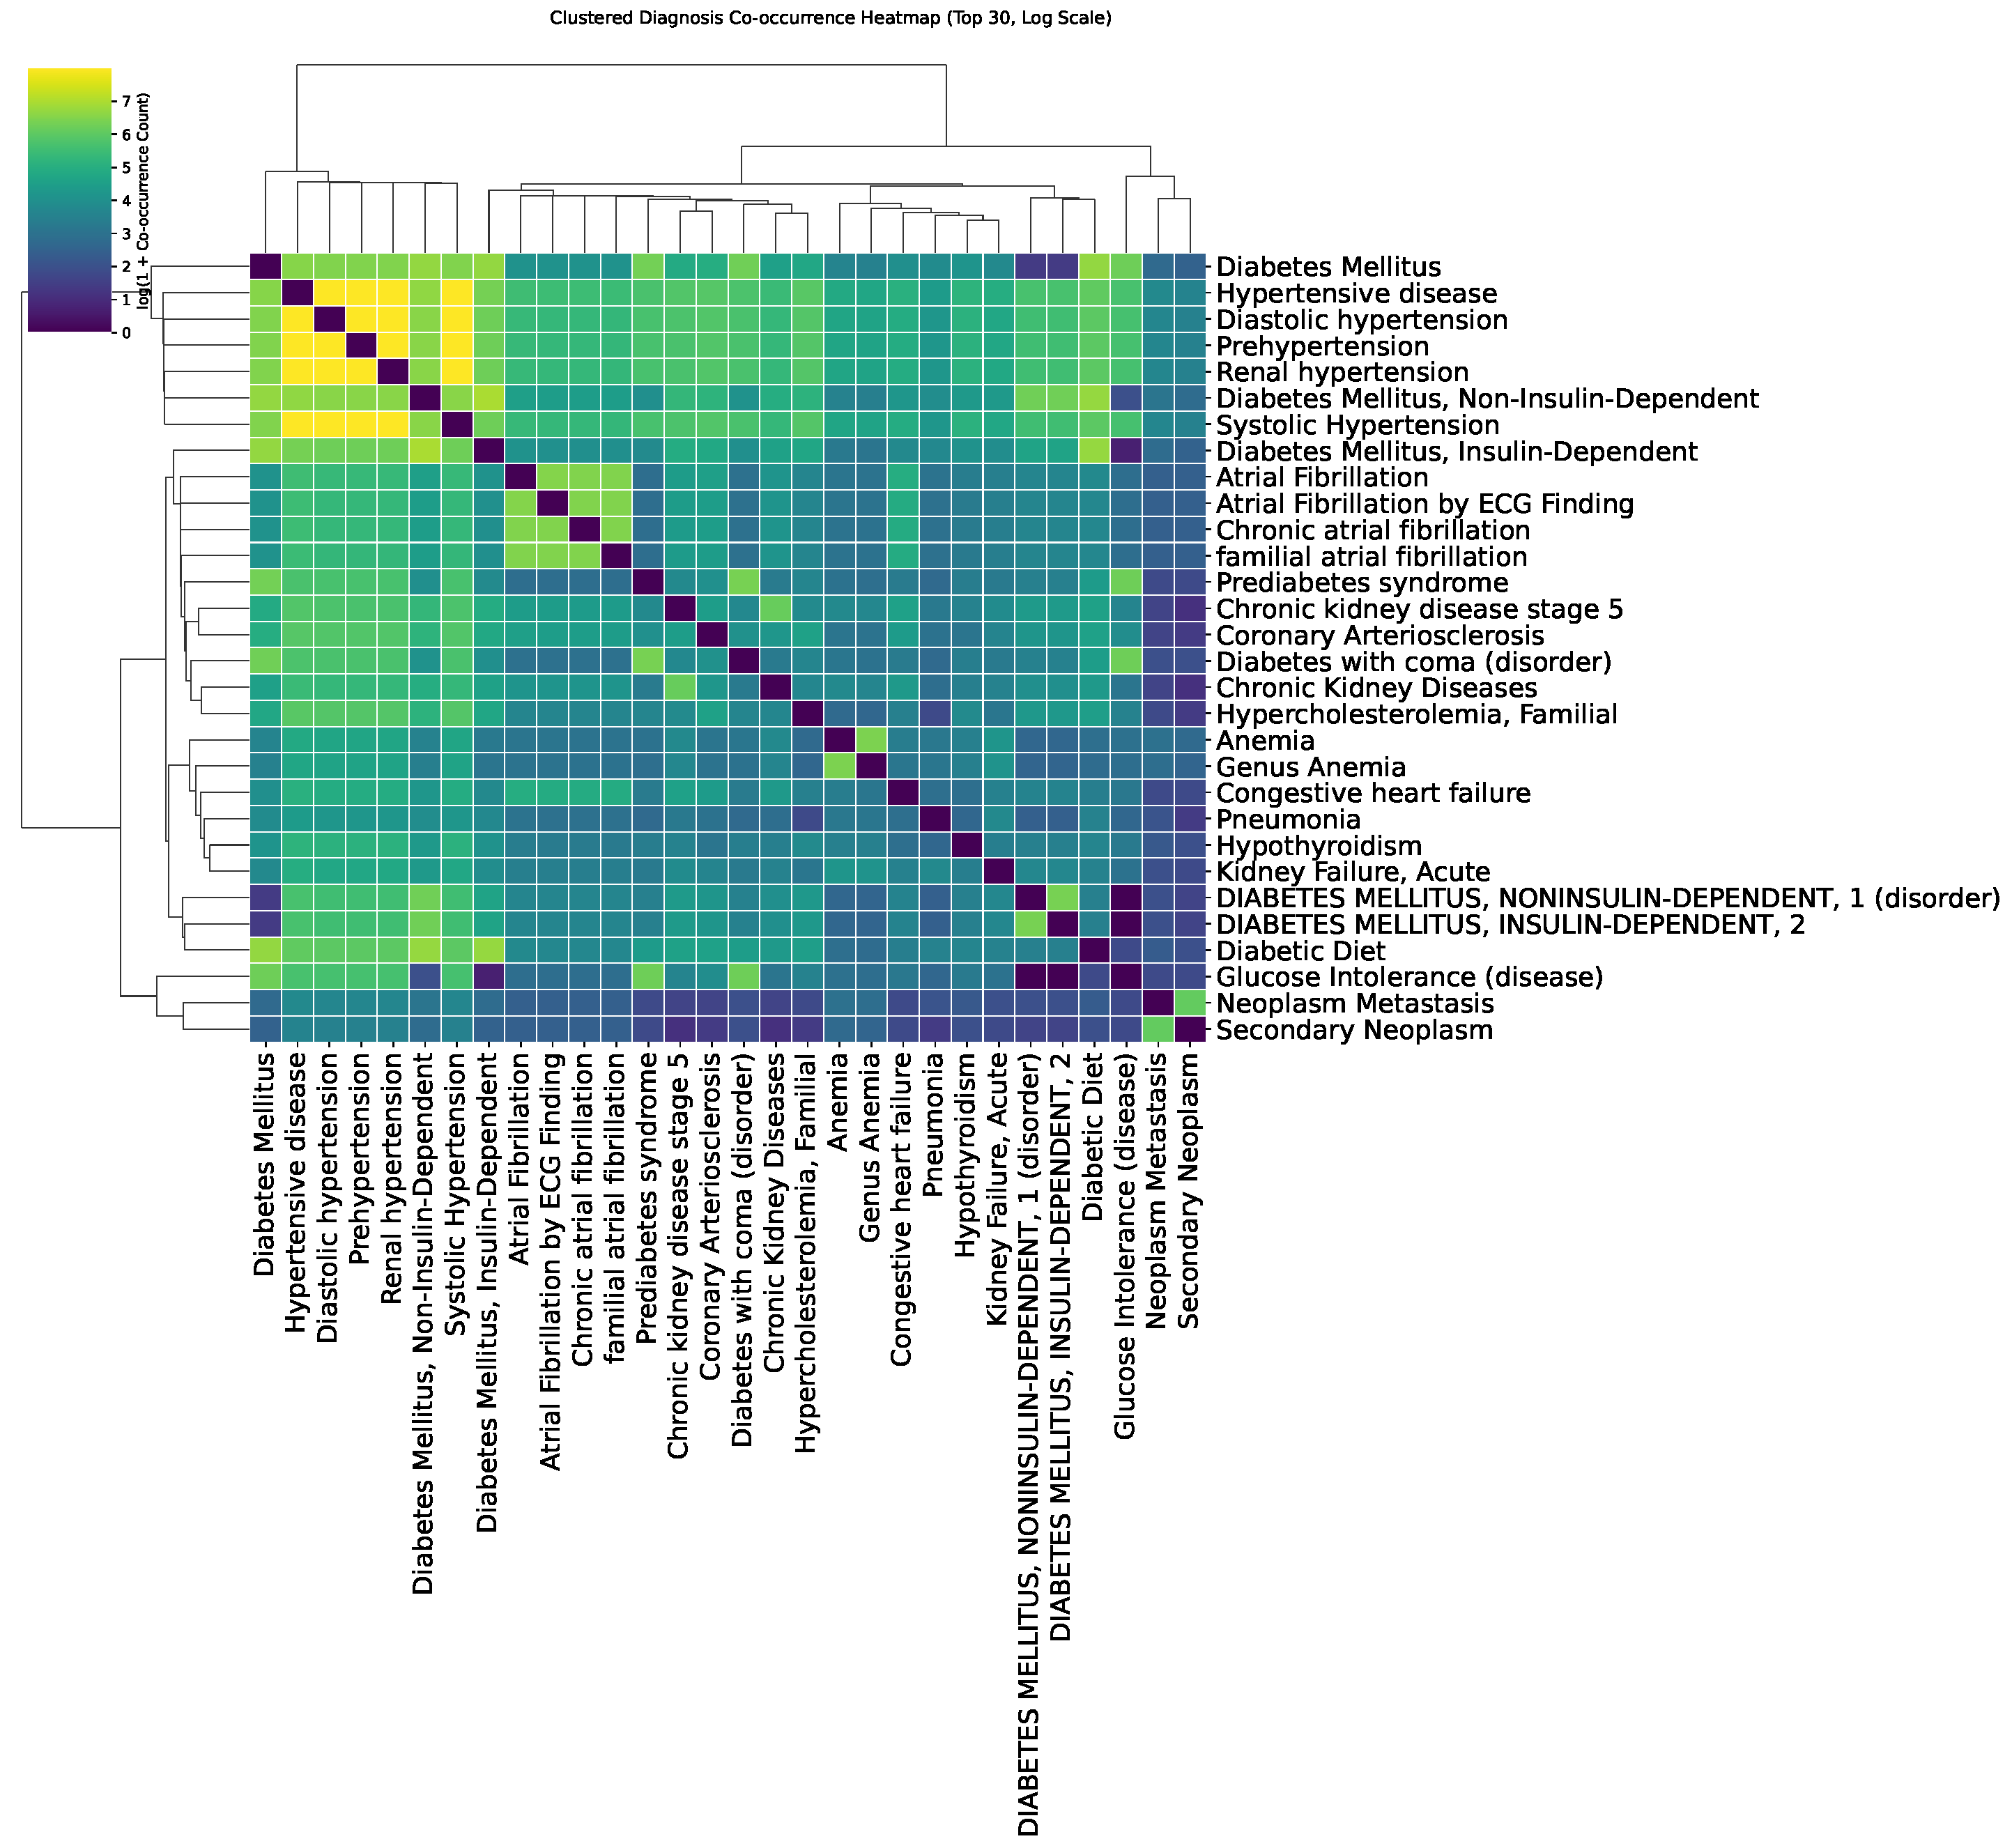
\includegraphics[width=0.99\linewidth]{Plots_tables/clustered_cooccurrence_heatmap_top30.pdf}
        \caption{Diagnoses Co-occurrence Heatmap in PMOA-TTS}
        \label{fig:diagnosis_cooccurrence}
        % \caption{}
    \end{subfigure}
    \caption{Co-occurrence Patterns and Frequency of Diagnoses in Clinical Case Reports. 
    The left panel shows the top 20 most frequently mentioned diagnoses, using UMLS canonical names, across clinical case reports. Cardiovascular and metabolic conditions such as hypertension, diabetes mellitus, and chronic kidney disease dominate the list. The right panel is a heatmap with hierarchical clustering, visualizing pairwise co-occurrence patterns (log-transformed counts) among diagnoses. Off-diagonal values reveal common comorbidity patterns in our PMOA-TTS. Clustering reveals distinct groups of frequently co-mentioned conditions, such as cardiovascular disorders and diabetes-related terms.}
    \label{fig:diagnoses}
    \vspace{-10pt}
\end{figure}


%\subsection{Downstream Task Performance}

\subsection{Survival Analysis Results}

Table \ref{tab:survival_results} presents the performance of different language model embeddings and survival models in predicting patient outcomes across three time thresholds (0h, 24h, and 168h). We show results for the time-dependent concordance index, which measures the model's ability to correctly rank patients by their risk. 
Descriptive analysis is provided in Appendix \ref{apd:survival_analysis}.

Several important patterns emerge from our results.
Decoder-based models (DeepSeek, LLaMA) consistently outperform encoder-based models (BERT variants) across all time horizons and survival modeling approaches.
LLaMA-3.3-70B-Instruct delivers the strongest performance overall, achieving concordance indices above 0.82 in most scenarios.
Within each model family, larger architectures (e.g., 70B vs. 8B) generally yield superior results, suggesting that greater model capacity enhances embedding quality for downstream survival prediction. Regarding observation windows, predictions that incorporate longer time spans (24h, 168h) show modest gains over the baseline (0h), indicating that additional temporal context contributes to improved prognostic accuracy, albeit with a relatively small effect.
In terms of survival modeling frameworks, DeepSurv and DeepHit exhibit comparable performance across most conditions, with no consistent advantage for either method.

Overall, these findings indicate that high-quality embeddings from LLMs can effectively encode prognostic signals from textual time series, with decoder-based models in particular showing strong potential for survival prediction tasks.

\begin{table}[!tbp]
% \vspace{-5pt}
\caption{Time-dependent concordance (mean ± standard deviation across 5 experimental runs) index across embedding models and survival modeling approaches at different time thresholds.} 
\label{tab:survival_results}
\centering
\begin{adjustbox}{width=\textwidth}
\begin{tabular}{lcccccc}
\toprule
\multirow{2}{*}{Embedding Model} & \multicolumn{2}{c}{Time Threshold = 0h} & \multicolumn{2}{c}{Time Threshold = 24h} & \multicolumn{2}{c}{Time Threshold = 168h} \\
\cmidrule(lr){2-3} \cmidrule(lr){4-5} \cmidrule(lr){6-7}
 & DeepHit & DeepSurv & DeepHit & DeepSurv & DeepHit & DeepSurv \\
\midrule
DeepSeek-R1-Distill-Llama-70B & 0.815 ± 0.010 & 0.812 ± 0.013 & 0.815 ± 0.012 & 0.818 ± 0.009 & 0.810 ± 0.012 & 0.812 ± 0.014 \\
DeepSeek-R1-Distill-Llama-8B & 0.806 ± 0.015 & 0.803 ± 0.011 & 0.809 ± 0.013 & 0.806 ± 0.011 & 0.802 ± 0.010 & 0.809 ± 0.011 \\
Llama-3.1-8B-Instruct & 0.815 ± 0.008 & 0.813 ± 0.010 & 0.817 ± 0.010 & 0.811 ± 0.007 & 0.808 ± 0.014 & 0.809 ± 0.011 \\
Llama-3.3-70B-Instruct & \textbf{0.822 ± 0.004} & \textbf{0.817 ± 0.011} & \textbf{0.821 ± 0.011} & \textbf{0.819 ± 0.005} & \textbf{0.819 ± 0.009} & \textbf{0.822 ± 0.009} \\
ModernBERT-base & 0.718 ± 0.011 & 0.729 ± 0.008 & 0.733 ± 0.010 & 0.738 ± 0.011 & 0.725 ± 0.013 & 0.729 ± 0.009 \\
ModernBERT-large & 0.653 ± 0.014 & 0.667 ± 0.009 & 0.655 ± 0.015 & 0.665 ± 0.017 & 0.643 ± 0.011 & 0.662 ± 0.003 \\
bert-base-uncased & 0.743 ± 0.013 & 0.746 ± 0.009 & 0.750 ± 0.014 & 0.748 ± 0.006 & 0.744 ± 0.009 & 0.747 ± 0.010 \\
deberta-v3-small & 0.739 ± 0.010 & 0.753 ± 0.010 & 0.730 ± 0.019 & 0.758 ± 0.006 & 0.733 ± 0.012 & 0.751 ± 0.006 \\
roberta-base & 0.757 ± 0.017 & 0.756 ± 0.013 & 0.760 ± 0.012 & 0.758 ± 0.014 & 0.761 ± 0.009 & 0.762 ± 0.011 \\
\bottomrule
\end{tabular}
\end{adjustbox}
\vspace{-1.5em}
\end{table}